\section{Two-Layer Process Architecture}
\label{sec_system_architecture}
Based on Section~\ref{sec_profile_us}, we find there too many factors to consider thus make problem too complex to solve. 
Thus, we propose a \textbf{two-layer process architecture} to simplify the problem without loss of generality.

In this section, we give a brief introduction to the two-layer process architecture we used to process this problem.
The main idea of this two-layer process architecture is to divide the whole problem into two dimension (\ie, Selection and Optimization).
Thus, we can classify various factors into two different layers so that we can simplify our model without loss of generality and make it solvable.
Figure 5 illustrates the Two-Layer Process Architecture in our paper.
\subsection{Selection Layer}
In Selection Layer,
the main task is to select the potential sites for charging stations.
This part mainly depends on many external factors (\eg, different geographies, population density, wealth distribution, policy of the government, area's type......).
Thus, we can just consider those factors in this layer.
After process, this layer should output the set of potential sites which can construct charging station.
%When we are trying to determine a specific location for constructing a new charing station within urban area, several potential locations have to be determined in the first place.
%A schematic elaborating this 2 step process has been depicted as follows.

\begin{figure}[!t]
\label{fig_system_architecture}
\centering
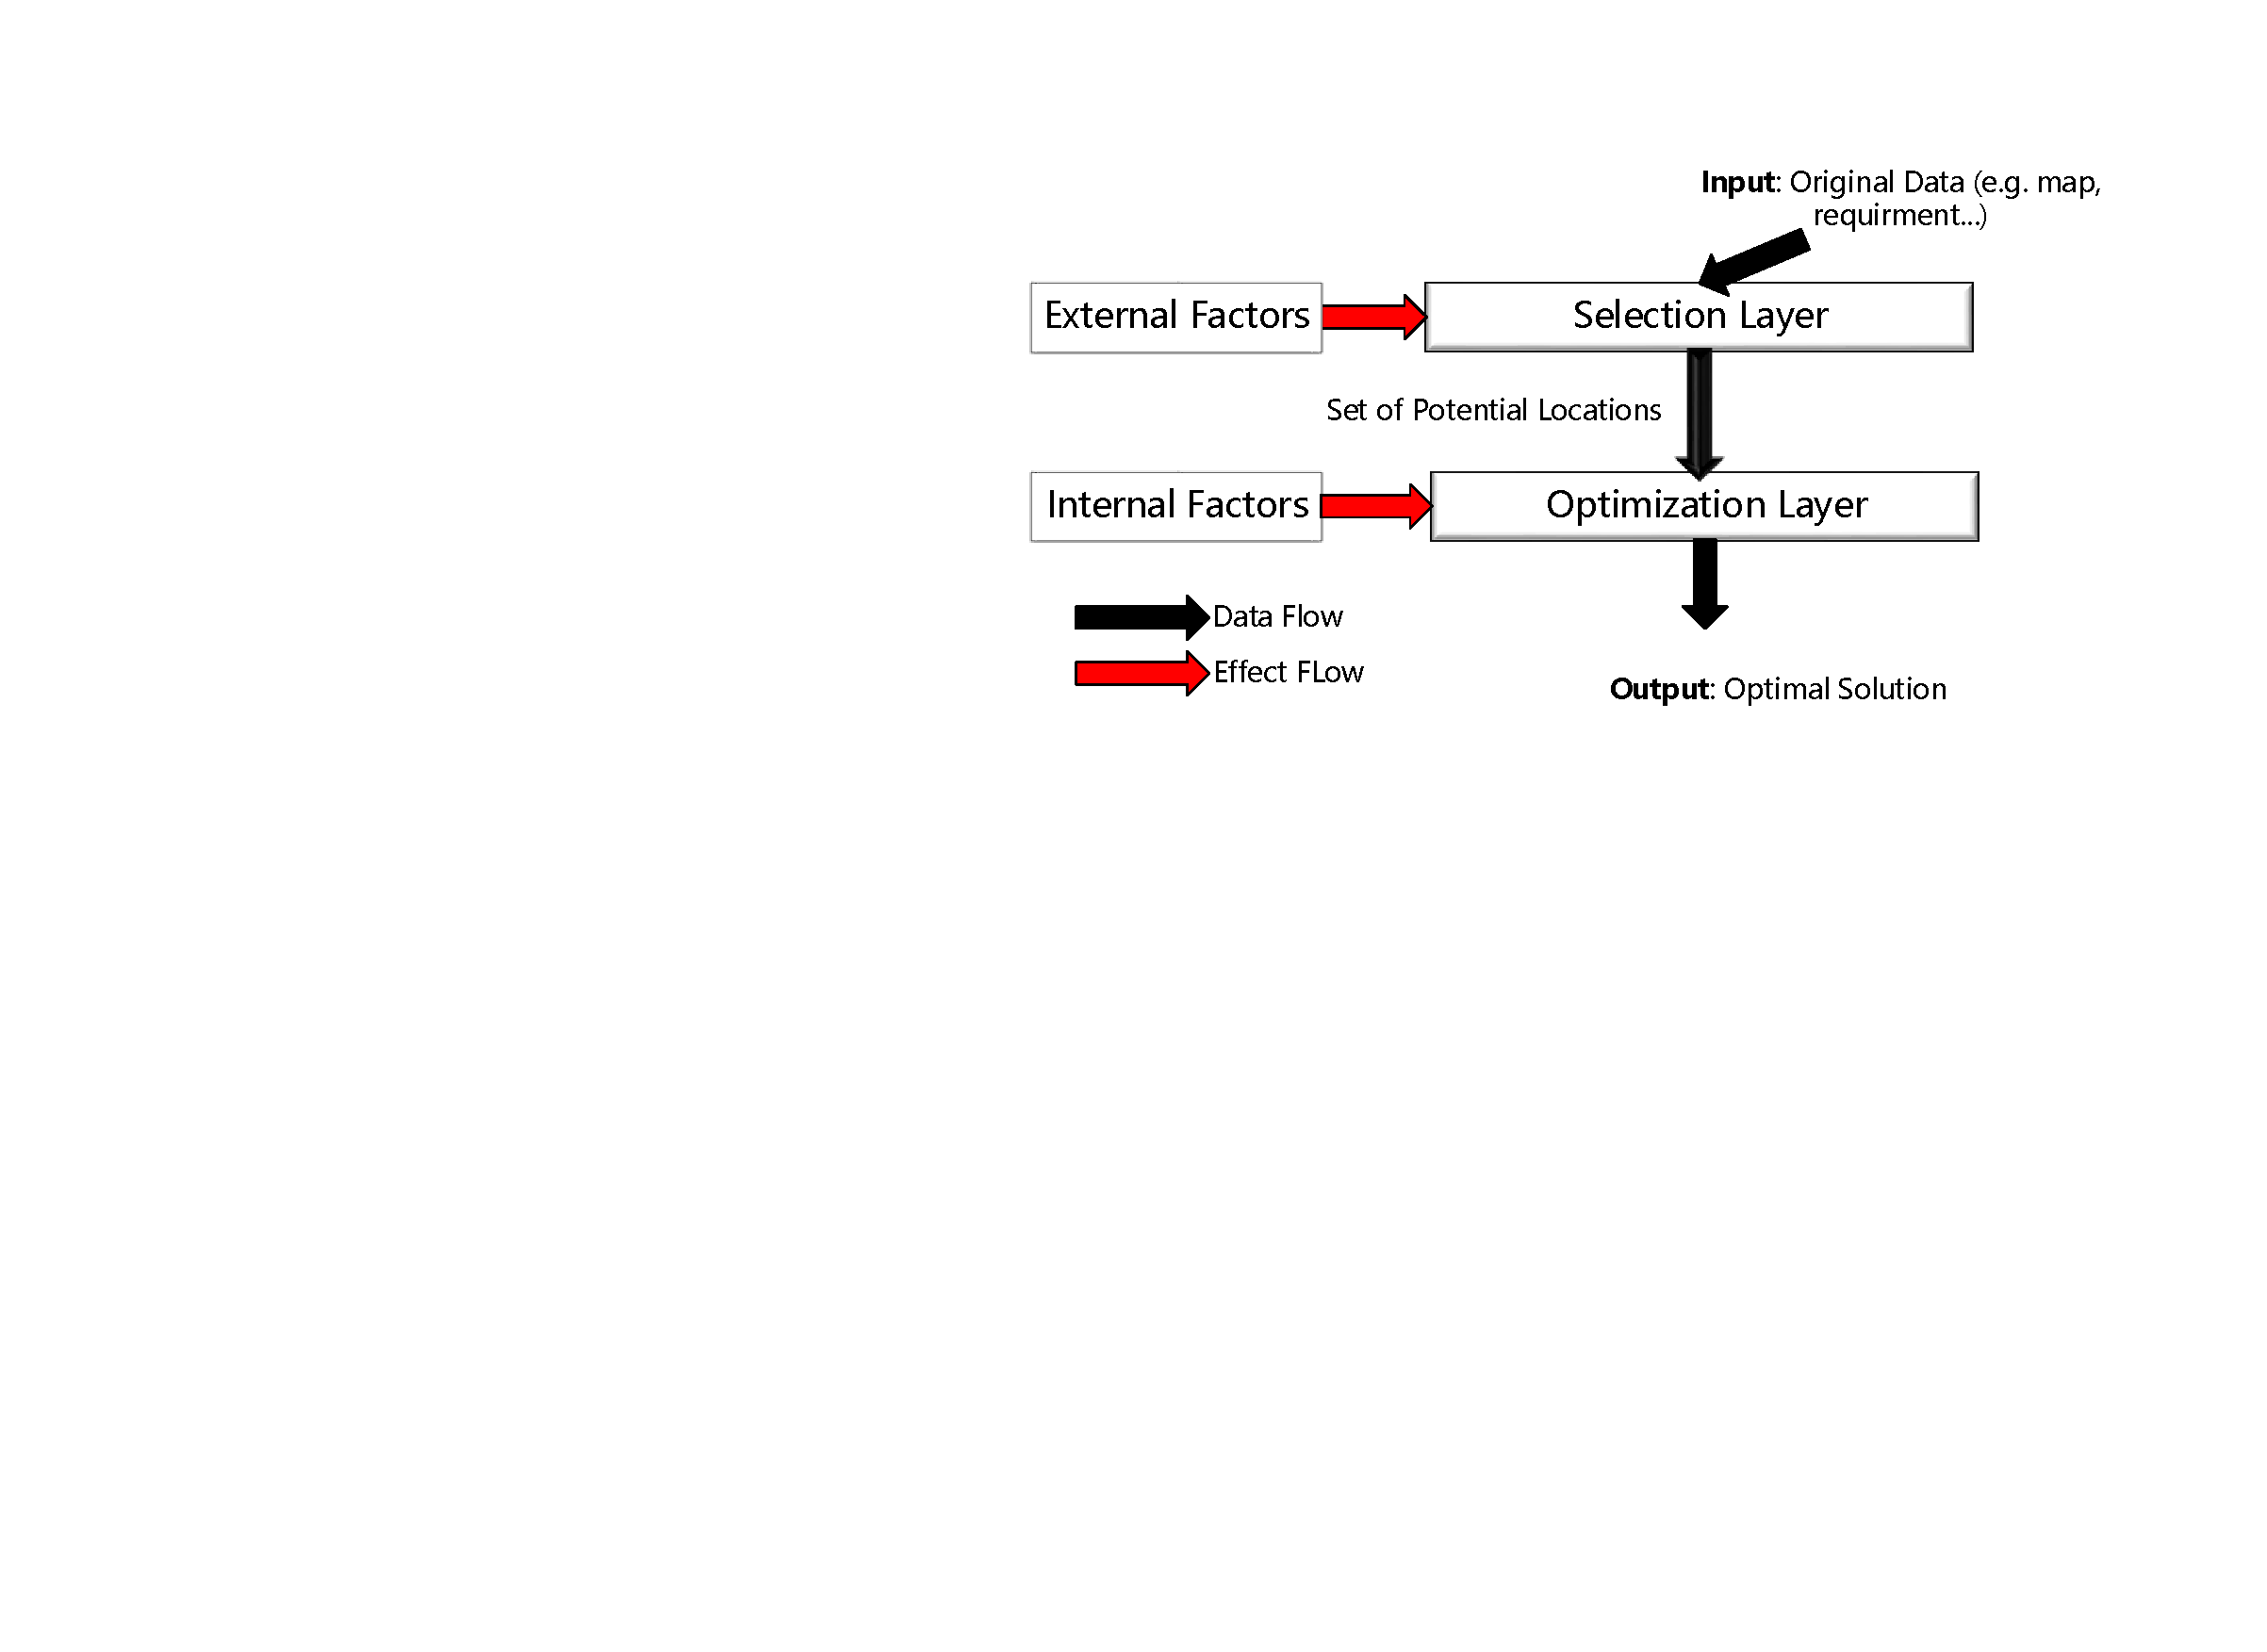
\includegraphics[width=4in]{system_architecture}
%\vspace{-0.1in}
\caption{Two-Layer Process Architecture}
%\vspace{-0.2in}
\end{figure}


\subsection{Optimization Layer}
In Optimization Layer,
the main task is to find the optimal number, placement, and distribution of charging stations based on the result from Selection Layer.
Since the set of potential sites is decided in Selection Layer,
according to the algorithm we designed in Section~\ref{sec_solve_optimal}, 
Optimization Layer just choose some sites of the set to achieve the optimal performance.
The algorithm depends on some internal factors (\eg, charging demand, the habit of drivers, connection of roads, service capacity of the charging station).
Therefore, we just consider those internal factors in this layer.
